\begin{figure}[H]
  \centering
  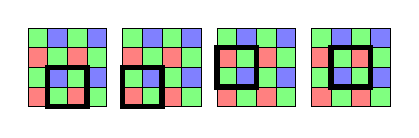
\begin{tikzpicture}
    \begin{scope}[shift={(0,0)}]
      \fill[fill=green!50](.25,0)   rectangle (.5,.25);
      \fill[fill=green!50](0,.25)   rectangle (.25,.5);
      \fill[fill=green!50](.75,.5)  rectangle (1,.75);
      \fill[fill=green!50](.5,.75)  rectangle (.75,1);

      \fill[fill=green!50](.75,0)   rectangle (1,.25);
      \fill[fill=green!50](.5,.25)  rectangle (.75,.5);
      \fill[fill=green!50](.25,.5)  rectangle (1,.75);
      \fill[fill=green!50](0,.75)   rectangle (.75,1);

      \fill[fill=red!50]  (0,0)     rectangle (.25,.25);
      \fill[fill=red!50]  (.5,0)    rectangle (.75,.25);
      \fill[fill=red!50]  (.5,.5)   rectangle (.75,.75);
      \fill[fill=red!50]  (0,.5)    rectangle (.25,.75);

      \fill[fill=blue!50] (.25,.25) rectangle (.5,.5);
      \fill[fill=blue!50] (.75,.25) rectangle (1,.5);
      \fill[fill=blue!50] (.25,.75) rectangle (.5,1);
      \fill[fill=blue!50] (.75,.75) rectangle (1,1);
      \draw[step=.25,very thin] (0,0) grid (1,1);

      \draw[line width=2pt] (.25, 0) rectangle (.75, .5);
    \end{scope}
    \begin{scope}[shift={(1.2,0)}]
      \fill[fill=green!50](.25,0)   rectangle (.5,.25);
      \fill[fill=green!50](0,.25)   rectangle (.25,.5);
      \fill[fill=green!50](.75,.5)  rectangle (1,.75);
      \fill[fill=green!50](.5,.75)  rectangle (.75,1);

      \fill[fill=green!50](.75,0)   rectangle (1,.25);
      \fill[fill=green!50](.5,.25)  rectangle (.75,.5);
      \fill[fill=green!50](.25,.5)  rectangle (1,.75);
      \fill[fill=green!50](0,.75)   rectangle (.75,1);

      \fill[fill=red!50]  (0,0)     rectangle (.25,.25);
      \fill[fill=red!50]  (.5,0)    rectangle (.75,.25);
      \fill[fill=red!50]  (.5,.5)   rectangle (.75,.75);
      \fill[fill=red!50]  (0,.5)    rectangle (.25,.75);

      \fill[fill=blue!50] (.25,.25) rectangle (.5,.5);
      \fill[fill=blue!50] (.75,.25) rectangle (1,.5);
      \fill[fill=blue!50] (.25,.75) rectangle (.5,1);
      \fill[fill=blue!50] (.75,.75) rectangle (1,1);
      \draw[step=.25,very thin] (0,0) grid (1,1);

      \draw[line width=2pt] (0, 0) rectangle (.5, .5);
    \end{scope}
    \begin{scope}[shift={(3.6,0)}]
      \fill[fill=green!50](.25,0)   rectangle (.5,.25);
      \fill[fill=green!50](0,.25)   rectangle (.25,.5);
      \fill[fill=green!50](.75,.5)  rectangle (1,.75);
      \fill[fill=green!50](.5,.75)  rectangle (.75,1);

      \fill[fill=green!50](.75,0)   rectangle (1,.25);
      \fill[fill=green!50](.5,.25)  rectangle (.75,.5);
      \fill[fill=green!50](.25,.5)  rectangle (1,.75);
      \fill[fill=green!50](0,.75)   rectangle (.75,1);

      \fill[fill=red!50]  (0,0)     rectangle (.25,.25);
      \fill[fill=red!50]  (.5,0)    rectangle (.75,.25);
      \fill[fill=red!50]  (.5,.5)   rectangle (.75,.75);
      \fill[fill=red!50]  (0,.5)    rectangle (.25,.75);

      \fill[fill=blue!50] (.25,.25) rectangle (.5,.5);
      \fill[fill=blue!50] (.75,.25) rectangle (1,.5);
      \fill[fill=blue!50] (.25,.75) rectangle (.5,1);
      \fill[fill=blue!50] (.75,.75) rectangle (1,1);
      \draw[step=.25,very thin] (0,0) grid (1,1);

      \draw[line width=2pt] (.25, .25) rectangle (.75, .75);
    \end{scope}
    \begin{scope}[shift={(2.4,0)}]
      \fill[fill=green!50](.25,0)   rectangle (.5,.25);
      \fill[fill=green!50](0,.25)   rectangle (.25,.5);
      \fill[fill=green!50](.75,.5)  rectangle (1,.75);
      \fill[fill=green!50](.5,.75)  rectangle (.75,1);

      \fill[fill=green!50](.75,0)   rectangle (1,.25);
      \fill[fill=green!50](.5,.25)  rectangle (.75,.5);
      \fill[fill=green!50](.25,.5)  rectangle (1,.75);
      \fill[fill=green!50](0,.75)   rectangle (.75,1);

      \fill[fill=red!50]  (0,0)     rectangle (.25,.25);
      \fill[fill=red!50]  (.5,0)    rectangle (.75,.25);
      \fill[fill=red!50]  (.5,.5)   rectangle (.75,.75);
      \fill[fill=red!50]  (0,.5)    rectangle (.25,.75);

      \fill[fill=blue!50] (.25,.25) rectangle (.5,.5);
      \fill[fill=blue!50] (.75,.25) rectangle (1,.5);
      \fill[fill=blue!50] (.25,.75) rectangle (.5,1);
      \fill[fill=blue!50] (.75,.75) rectangle (1,1);
      \draw[step=.25,very thin] (0,0) grid (1,1);

      \draw[line width=2pt] (0, .25) rectangle (.5, .75);
    \end{scope}
  \end{tikzpicture}
  \caption{CFA augmentation cropping a GRBG sensor to other layouts.}
  \label{fig:cfaaug}
\end{figure}